\chapter{Background} \label{ch:background}

This chapter provides an overview of the problem of portfolio optimisation in the financial domain, followed by a comprehensive explanation of the fundamentals of \acrfull{dl} and \acrfull{rl}, including the relevant algorithms in the field of \acrfull{drl}. In addition, it discusses the need for explainability in \acrfull{ml} and the main techniques used to achieve it: \acrfull{shap}, \acrfull{lime} and \Gls{featureimportance}. Finally, it presents the state of the art in portfolio optimisation using \acrshort{drl} and the recent advancements in explainability techniques in the field. 

\section{Portfolio Optimisation} \label{sec:portfoliooptimisation}

\Gls{portfoliooptimisation} is the process of selecting optimal weights for a portfolio of assets in order to maximise expected returns for a given level of risk, or conversely, to minimise risk for a given level of expected returns \cite{Sato2019}. In mathematical terms, the problem requires finding a solution to the specified objective function, which is typically a function of the expected returns and the risk associated with the portfolio \cite{Bruce2014}. The task becomes further complicated if a time dimension is introduced, as the portfolio weights need to be adjusted over time to capture the changes in market conditions and asset prices \cite{Li2019}. 

\subsection{Modern Portfolio Theory}

There exist several traditional frameworks that formalise the problem of portfolio allocation. Markowitz's \acrfull{mpt} was proposed in 1952 \cite{Markowitz1952} and it provides a mathematical framework where investors choose optimal portfolios based on risk and return, by either minimising the risk given a specified return or, maximising the return given a specified risk \cite{kent}. The theory extends the concept of diversification by suggesting that owning financial assets of different kinds is less risky than owning assets of the same kind, due to the correlations between assets. 

The main assumptions in \acrshort{mpt} are:
\begin{itemize}
    \item investors are risk-averse, rational, and seek to maximise return for a given risk;
	\item returns are normally distributed;
	\item markets are frictionless, meaning there are no transaction costs; and
	\item assets are infinitely divisible.
\end{itemize}

Under these assumptions, portfolio risk and return can be modelled as an optimisation problem. Let $\mathbf{w} = \left(w_1, w_2, \dots, w_N\right)^T$ denote the portfolio weight vector, where each $w_i$ indicates the proportion of capital allocated to asset $i$, subject to the budget constraint:
\begin{equation}
    \sum_{i=1}^{N} w_i = 1 \quad \Leftrightarrow \quad \mathbf{w}^T \mathbf{1} = 1
\end{equation}
with $\mathbf{1} \in \mathbb{R}^N$ being a vector of ones, and subject to the non-negativity constraint, meaning that short-selling is not allowed:
\begin{equation}
    w_i \geq 0 \quad \forall i = 1, 2, \dots, N.
\end{equation}

Let $\boldsymbol{\mu} = \left(R_1, R_2, \dots, R_N\right)^T$ represent the vector of expected returns, and $\Sigma \in \mathbb{R}^{N \times N}$ the covariance matrix of asset returns. The expected return of the portfolio is then given by:
\begin{equation}
    R_p = \mathbf{w}^T \boldsymbol{\mu},
\end{equation}
and the portfolio risk is quantified by the variance of returns:
\begin{equation}
    \sigma_p^2 = \mathbf{w}^T \Sigma \mathbf{w}.
\end{equation}


This formulation provides the foundation for solving the mean-variance optimisation problem, by either:
\begin{itemize}
    \item minimising portfolio variance $\sigma_p^2$ subject to a target expected return $R_p$, or
    \item maximising expected return $R_p$ subject to a risk constraint $\sigma_p$.
\end{itemize}

The Markowitz mean-variance optimisation problem can be expressed as:
\begin{equation}
\begin{aligned}
    \min_{\mathbf{w}} \quad & \mathbf{w}^T \Sigma \mathbf{w} \\
    \text{subject to} \quad &
    \begin{cases}
        \mathbf{w}^T \boldsymbol{\mu} = R_p \\
        \mathbf{w}^T \mathbf{1} = 1 \\
        \mathbf{w} \geq 0
    \end{cases}
\end{aligned}
\end{equation}

Solving the mean-variance optimisation problem for varying levels of target return leads to a set of optimal portfolios that form the \gls{efficientfrontier}. It is typically visualised in a risk-return space, where the x-axis represents the risk (standard deviation) and the y-axis represents the expected return, as shown in Figure \ref{fig:efficient_frontier}. Portfolios below the curve are suboptimal, while those on the frontier represent the best achievable combinations of risk and return.

\begin{figure}[h]
    \centering
    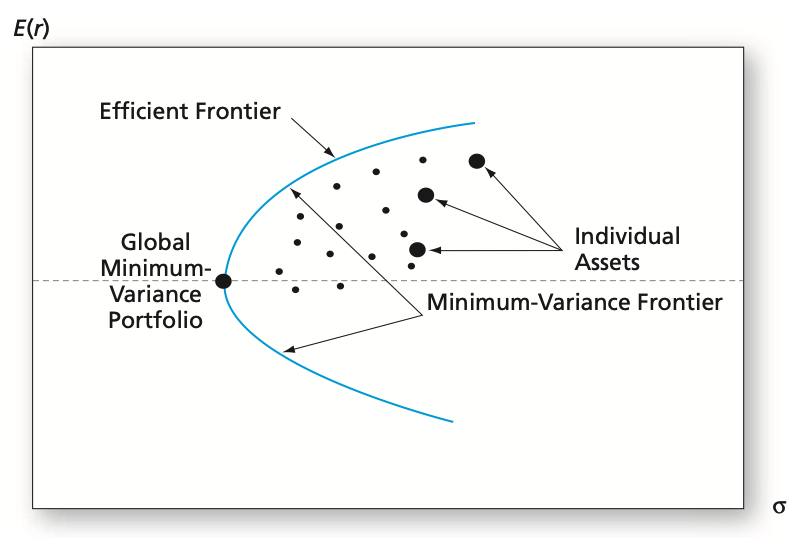
\includegraphics[width=0.8\textwidth]{figures/markowitz-efficient-frontier.png}
    \caption{Efficient Frontier in Risk-Return Space. \cite{Bodie2014}}
    \label{fig:efficient_frontier}
\end{figure}

Despite the simplicity in the formulation of \acrshort{mpt}, its assumptions do not reflect the behaviour of real markets. Moreover, modern markets are dynamic, non-stationary, and feature non-linear relationships, which have driven research into other approaches better suited to capture the complexities of modern financial markets. 
